\lab{Algorithms}{Krylov Subspaces}{Finding Eigenvalues Using Iterative Methods}
\label{lab:kry_arnoldi}

\objective{Discuss simple Krylov Subspace Methods for finding eigenvalues and show some interesting applications.}

In the realm of numerical linear algebra, Krylov Subspace Methods are considered some of the most successful  methods ever invented.
They are simple and robust and can be used to find approximate solutions to linear systems and eigenvalue problems involving extremely
large matrices.
One of the reasons for this success is that they do not require copies or modifications of the original
matrix.
Krylov subspace methods are used to estimate certain properties of a matrix based on how it acts on vectors through matrix multiplication.
This is especially useful for large sparse matrices (allowing us to deal with the matrix in compressed form),
and for matrices that have symmetries that reduce storage and enable faster matrix multiplication (allowing us to use
specialized algorithms like the Fast Fourier Transform rather than the full matrix).

The general approach of Krylov subspace methods is to consider how a given matrix $A$ acts on the span of
$\{ x, Ax, A^2 x, \ldots, A^{N-1} x \}$ (called an \emph{order-$N$ Krylov Subspace generated by $A$ and $x$}), where $N$ is significantly
smaller than the number of rows of $A$.
The formation of these subspaces in an efficient and numerically stable manner is usually based on either the \emph{Arnoldi
iteration} or the \emph{Lanczos iteration}. We will discuss both of these algorithms here.

\section*{The Arnoldi Iteration}

Before discussing the specific uses of the Krylov subspace in linear systems and eigenvalue problems, let us address a very
practical concern: how can we best compute a basis for the Krylov subspace? The obvious answer is simply to
calculate the vectors $x, Ax, A^2x, \ldots, A^{N-1} x$, which we can accomplish using only matrix-vector multiplication.
Straightforward though this may be, there is a major problem: $A^n x$ tends to converge to a dominant eigenvector of $A$
as $n$ gets large, and consequently these vectors become nearly parallel. Thus, the basis $\{x, Ax, A^2x, \ldots, A^{N-1} x\}$
is far from orthogonal, and matrix computations associated with this basis will likely be ill-conditioned and prone to
numerical instability. To redress this problem, we may think to apply the Gram-Schmidt orthogonalization process to the
basis, obtaining an orthonormal basis for the Krylov subspace that enjoys much better numerical properties. This turns out to
be a useful thought, and is the basis for the Arnoldi iteration.

You may recall from lab \ref{lab:QRdecomp} that the Modified Gram-Schmidt algorithm allows us to find an increasing number of orthogonal
vectors but does not require that we run the algorithm to is completion to find a full basis.
Our goal is to find an orthonormal set of vectors $q_1,\ldots,q_N$ having the same span as $x, Ax, A^2x, \ldots, A^{N-1} x$.
We start
 things off by setting
\[
q_1 = \frac{x}{\|x\|_2}.
\]
Now, assuming we have obtained $q_1,\ldots,q_n$, we obtain $q_{n+1}$ by projecting $A q_n$ onto the previous vectors,
subtracting out these projections, and then normalizing. To make this more precise, let $h_{i,n} = \langle q_i, A q_n\rangle$
for $i = 1,\ldots, n$. Subtract out these projections by calculating
\[
p_{n+1} = A^n x - \sum_{i=1}^n h_{i,n}q_i.
\]
Define $h_{n+1,n} = \|p_{n+1}\|_2$, and normalize $p_{n+1}$ by calculating
\[
q_{n+1} = \frac{p_{n+1}}{h_{n+1,n}},
\]
our next basis vector. This procedure is outlined (in slightly more Python-friendly notation) in Algorithm \ref{alg:arnoldi_iteration}.

Perhaps you noticed a slight discrepancy between the Arnoldi iteration as described above, and the usual Gram-Schmidt procedure.
Specifically, you might have expected to compute $q_{n+1}$ by projecting $A^n x$, rather than $A q_n$, onto the previous vectors.
Thankfully, it is straightforward to show that our algorithm produces a valid orthonormal basis for the Krylov subspace,
despite this difference. And because of this detail, we do not need to compute and store the original Krylov basis
$x, Ax, \ldots, A^{N-1}x$.
Additionally, each iteration only requires one matrix-vector calculation, and the individual entries in $A$ are never
referenced or modified. Thus, even if the matrix $A$ is very large in theory, as long as we have a reasonably efficient
subroutine to calculate $Ax$ for any vector $x$, the Arnoldi iteration is computationally tractable.

This algorithm produces an othonormal basis $q_1,\ldots,q_N$ for the order-$N$ Krylov subspace generated by $A$ and $x$, as well
as a collection of numbers $h_{i,j}$. If we define a matrix $H_N$ whose $i,j$'th entry is $h_{i,j}$ for $i \leq j+1$ and
is $0$ otherwise, we now have an upper Hessenberg matrix.
Recall that an upper Hessenberg matrix has the property that all entries below the first subdiagonal
are equal to zero. Any square matrix is unitarily similar to an upper Hessenberg matrix. Dealing with a Hessenberg matrix is
often more convenient than dealing with a general matrix, especially when it comes to finding eigenvalues or solving systems
of equations, since efficient algorithms designed for these types of matrices exist.
It turns out that there is a Hessenberg factorization of $A$, given by
\[
A  = QHQ^*,
\]
where $Q$ is a unitary matrix and $H$ is upper Hessenberg such that the first $N$ columns of $Q$ are $q_1,\ldots,q_N$, and
the upper left $N \times N$ submatrix of $H$ is equal to $H_N$. Hence, the Arnoldi iteration provides a connection between
the Krylov subspace and the Hessenberg factorization of a matrix. Each step in the Arnoldi iteration can be thought of as computing
another step in the Hessenberg reduction of $A$. Each $H_N$ is really just the $N \times N + 1$ upper-left block of $H$.
Solving eigenvalue problems or systems of equations for
a general square matrix can thus be reduced, via Arnoldi iteration, to solving these problems for a Hessenberg matrix,
a much easier task.

At this point, we can view the Arnoldi iteration as a means to compute an orthonormal basis for a Krylov subspace, or
alternatively, to compute a partial Hessenberg factorization of a matrix.
But in Lab \ref{lab:Canonical_Transformations}, we discussed how orthogonal transformations can be used to transform a matrix to Upper
Hessenberg form.
We were able to find the eigenvalues of such Upper Hessenberg matrices in Lab \ref{lab:EigSolve}.
So what have we really gained by this new approach?
These previous approaches were based on matrix-matrix multiplication and required us to manipulate individual entries of the matrix.
The Arnoldi iteration avoids this and relies only on our ability to calculate matrix-vector multiplication.
Further, our present approach will allow us to compute only a partial Hessenberg factorization. This is advantageous when, as
is often the case, the behavior and properties of a matrix can be well-approximated by only a small portion of its Hessenberg
form.

%The idea is to construct a set of vectors that allow us to roughly approximate the action of a very large matrix on the subspace.
%This involves forming only a portion of the actual Hessenberg reduction of the Hessenberg factorization of the matrix.
%You may recall from lab \ref{lab:QRdecomp} that the Modified Gram-Schmidt algorithm allows us to find an increasing number of orthogonal
%vectors but does not require that we run the algorithm to is completion to find a full basis.
%In the Arnoldi iteration we use the Modified Gram-Schmidt algorithm to compute progressively larger portions of the matrices $Q$ and $H$
%in the Hessenberg factorization of $A$.
%These intermediate matrices often carry a significant amount of information about $A$, and we can get away with storing small portions of
%them instead of having to store a dense version of the matrix $A$.
%The Arnoldi iteration is outlined in Algorithm \ref{alg:arnoldi_iteration}.
%We will now consider the ideas underlying the Arnoldi iteration in further detail.
%
%Let $A$ be an extremely large matrix that we do not wish to modify.
%We will assume that we have some sort of method for computing $A v$ for any vector $v$, but we will not make any other assumptions
%relating to how $A$ is stored or what properties it has.
%Write the Hessenberg factorization of $A$ as
%\[
%Q^* A Q = H,
%\]
%where $Q$ is a unitary matrix and $H$ is Upper Hessenberg.
%
%We would like to compute the columns of $Q$ one-by-one.
%Let $q_k$ be the $k$'th column of $Q$ and $h_{i,j}$ be the $i,j$'th element of $H$.
%From matrix multiplication we have that
%\[A q_n = h_{0, n} q_0 + \dots + h_{n, n} q_n + h_{n+1, n} q_{n+1}\]
%This can be rewritten as
%\[h_{n+1, n} q_{n+1} = A q_n - h_{0,n} q_0 - \dots - h_{n,n} q_n\]
%Since each column of $Q$ has norm $1$, this allows computation of each $q_k$ based on each of the previous columns.
%This recurrence relation does not provide any constraint on the first column of $Q$.
%In practice, if we are searching for eigenvalues we can use a normalized random vector as the first column of $Q$.
%These columns of $Q$ allow compution of partial reductions of $A$ to Hessenberg form without any modification of $A$.
%This can seen as follows:
%
%Let $Q_k$ be the first $k$ columns of $Q$.
%Let $Q_u$ be the remaining columns of $Q$.
%We then have that
%\[H = Q^T A Q =
%\begin{bmatrix}
%Q_k^* A Q_k & Q_k^* A Q_u \\
%Q_u^* A Q_k & Q_u^* A Q_u
%\end{bmatrix}\]
%Since $H$ is Upper Hessenberg, so is the matrix $Q_k^* A Q_k$ in the upper left corner.
%Let $H_k = Q_k^* A Q_k$.
%Note that we really only need to store the columns of $Q$ that we have already computed.
%We can also construct the $H_k$ as we go.
%
%\begin{info}
%The recurrence relation for computing $q_{n+1}$ is the same expression that would be used to perform Gram-Schmidt orthogonalization
%to project $A q_n$ orthogonal to the vectors $\{ q_0, \dots, q_n \}$.
%This allows for an alternate characterization of the Arnoldi iteration.
%We first choose a normalized random vector $q_0$, then perform the Modified Gram-Schmidt algorithm on the vectors
%$A q_0, A q_1, A q_2, \dots$.
%\end{info}

\begin{algorithm}
\begin{algorithmic}[1]
\Procedure{arnoldi}{$b, Amul, k, tol=1E-8$}
	\State $m \gets b.size$						\Comment{Some initialization steps}
	\State $Q \gets \text{empty}\left(m, k+1\right)$
	\State $H \gets \text{zeros}\left( k+1, k\right)$
	\State $q_0 = b$							\Comment{Set $q_0$ equal to $b$.}
	\State $q_0 /= \|q_0\|_2$						\Comment{Normalize $q_0$.}
	\For{$j=0$, $j<k$}							\Comment{Perform the actual iteration.}
		\State $q_{j+1} = Amul \left(q_j\right)$		\Comment{Compute $A q_j$.}
		\For{$i=0$, $i<j+1$}					\Comment{Modified Gram-Schmidt.}
			\State $h_{i,j} = \langle q_i, q_{j+1}\rangle$		\Comment{Set values of $H$.}
			\State $q_{j+1} -= h_{i,j} q_i$
		\EndFor
		\State $h_{j+1,j} = \|q_{j+1}\|_2$			\Comment{Set subdiagonal element of $H$.}
            \If{$|h_{j+1,j}|<tol$}					\Comment{Stop if $\|q_{j+1}\|_2$ is too small.}
			\State \pseudoli{return} $H[:j,:j]$
		\EndIf
		\State $q_{j+1} /= h_{j+1,j}$				\Comment{Normalize $q_{j+1}$.}
	\EndFor
	\State \pseudoli{return} $H[:-1]$				\Comment{Return $H_{k}$.}
\EndProcedure
\end{algorithmic}
\caption{The Arnoldi Iteration}
\label{alg:arnoldi_iteration}
\end{algorithm}

\begin{warn}
To avoid errors involving the casting of complex numbers to real numbers make the datatypes of $H$ and $Q$ complex.
Make sure you account for the use of complex numbers when computing the norm.
You will also want to use the complex version of the \li{sqrt} function.
This function is in the built in \li{cmath} library.
\end{warn}

Notice that in Algorithm \ref{alg:arnoldi_iteration}, $k$ is the number of times to multiply by $A$.
This will result in a dimension $k+1$ Krylov Subspace.

\begin{problem}
Write a Python function that performs the Arnoldi iteration given a nonzero starting vector $b$, a function to multiply a
vector on the left by some matrix $A$, and a number $n$ of steps to perform.
Also have it accept a tolerance parameter that defaults to \li{1E-8}.
Have it return the computed $H_n$ and $Q_n$.
\end{problem}

\begin{info}
Depending on the matrix $A$, the Arnoldi iteration may end quickly.
This happens when there is a subspace $G$ that is fixed under left multiplication by $A$.
In this particular case, the matrix $H_k$ exactly matches the way $A$ acts on $G$.
This means that the eigenvalues of $H_k$ are eigenvalues of $A$.
The eigenvectors of $H$ will also be eigenvectors of $A$ after the change of basis defined by $Q_k$.
\end{info}

% Make a 3D plot showing the projection. Label the initial vector x and Ax.

\section*{Finding Eigenvalues Using Arnoldi iteration}

It is relatively easy to understand how Arnoldi iteration finds eigenvalues of a matrix.
In simple terms, the eigenvalues of the $H_k$ converge to the eigenvalues of $A$.
The eigenvalues of the $H_k$ are called Ritz values.
This can happen very quickly, but, in general, the rate of convergence depends on the matrix $A$.
This works because each $H_k$ is a kind of lower-dimensional approximation of $A$.
In adding the projection of $A q_n$ orthogonal to $q_0, \ldots, q_n$, we are really including the only portion
of the space spanned by the image of $q_0, \dots, q_n$ under $A$ that is not already included in their span.
Generally speaking, the Ritz values converge most quickly to the eigenvalues of largest magnitude.
Convergence is also faster for eigenvalues that are relatively far from the other eigenvalues of $A$.
Figures \ref{fig:arnoldi_random_eig_conv} and \ref{fig:arnoldi_random_val_conv} show the convergence of the
Ritz values to the largest eigenvalues of some different matrices.

\begin{figure}
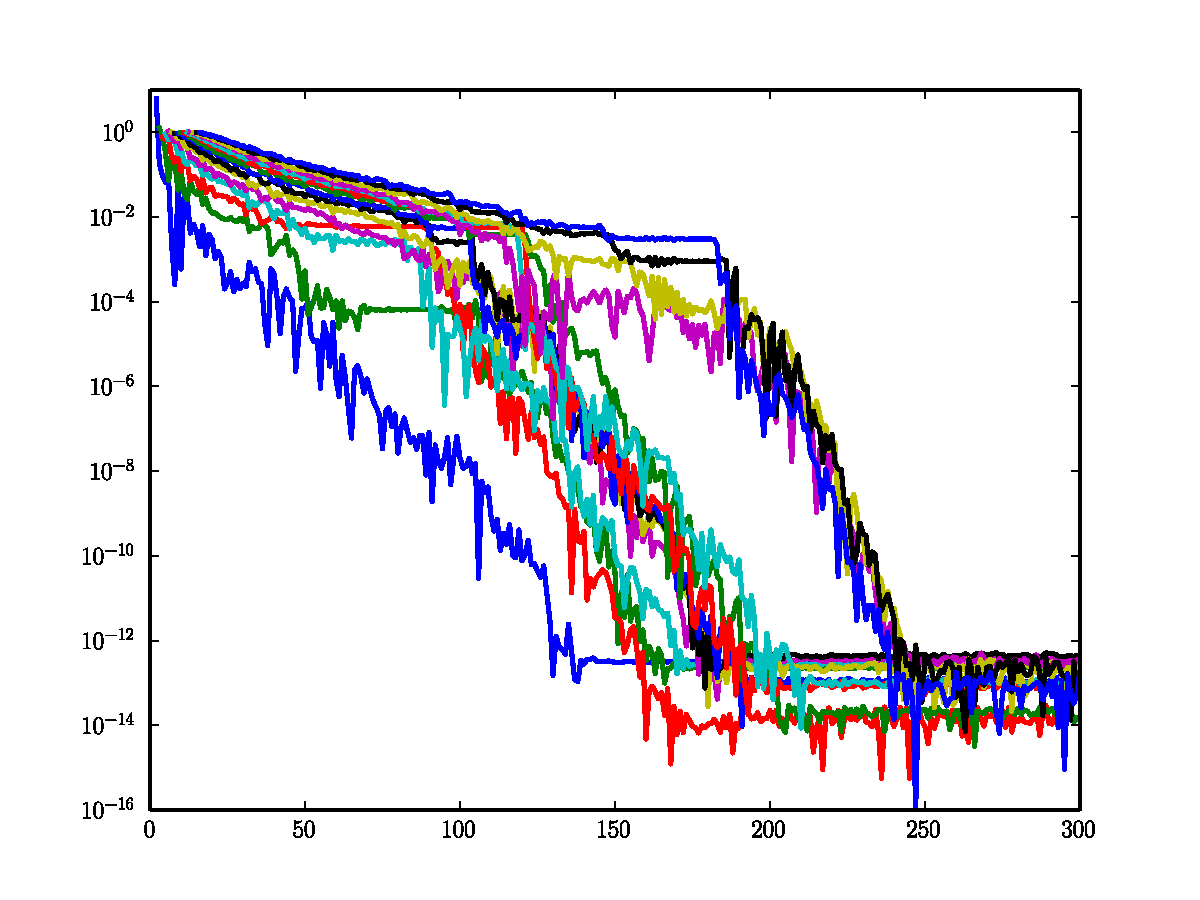
\includegraphics[width=\textwidth]{rand_eigs_conv.pdf}
\caption{The convergence of the Ritz values to the largest eigenvalues of a matrix with random eigenvalues between $0$ and $1$.}
\label{fig:arnoldi_random_eig_conv}
\end{figure}

\begin{figure}
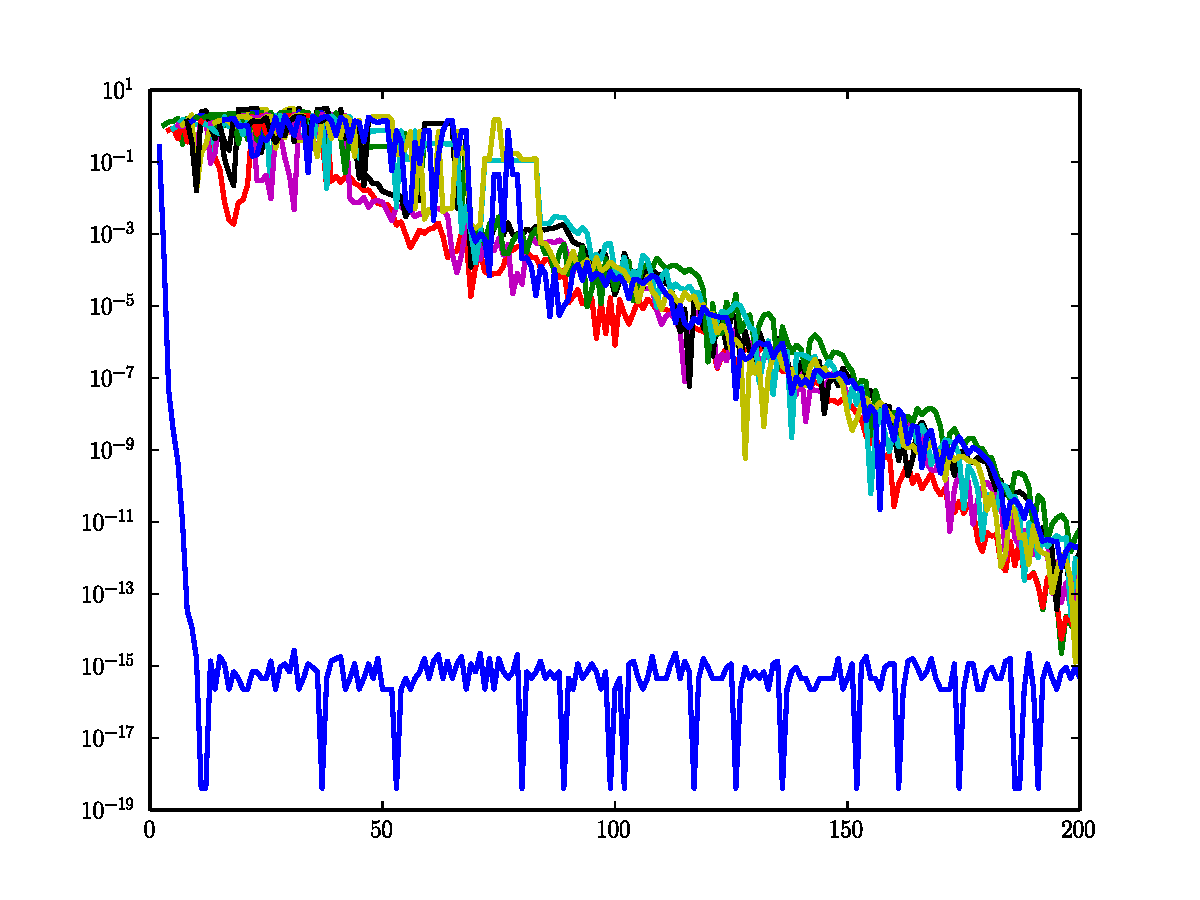
\includegraphics[width=\textwidth]{rand_vals_conv.pdf}
\caption{The convergence of the Ritz values to the largest eigenvalues of a matrix with random entries between $0$ and $1$.
Matrices of this form generally have a single isolated eigenvalue that is much larger than the rest.
It can be seen here that the Ritz values converge to this eigenvalue much more quickly.}
\label{fig:arnoldi_random_val_conv}
\end{figure}

\begin{problem}
Run the Arnoldi iteration on a random $100 \times 100$ array $A$.
Use a random vector as a starting point.
Find $H_{40}$ and compare the $10$ eigenvalues of largest magnitude of $H_{40}$ with the $10$ eigenvalues of largest magnitude of $A$.
Arnoldi iteration is not the most effective way to work with dense matrices without significant patterns, but this example does illustrate the desired convergence.
\end{problem}

\begin{problem}
\label{prob:fourier_eigs}
The Discrete Fourier Transform is a linear operator, so it has a matrix representation.
This matrix representation is well known and the symmetries that arise in it are used in computing the Fast Fourier Transform.
Fast Fourier Transforms are discussed in much greater detail in Volume 2.

Since the Fast Fourier Transform is a linear operator, it also has eigenvalues and eigenvectors.
The eigenvalues are known to be $\{ -1, 1, -i, i \}$.
Use your implementation of the Arnoldi iteration to estimate the eigenvalues of the Discrete Fourier Transform.
This can be done by passing the \li{fft} function from either \li{pyfftw.interfaces.scipy_fftpack} or \li{scipy.fftpack} as the argument \li{Amul} to your function for the Arnoldi iteration.
Let $b$ be a random real-valued array of size $2^{20}$.
Let $k = 10$.
You will need to either divide your computed eigenvalues or your computed value for each $A q_i$ by $2^{10}$ (the square root of the length of $b$).
This is a normalizing factor that comes from the way the Fast Fourier Transform is defined.

All the eigenvalues of the Discrete Fourier Transform should show up most of the times this code is run.
\end{problem}

Problem \ref{prob:fourier_eigs} shows how Arnoldi Iteration works nicely on matrices with useful patterns.
What is remarkable is that the matrix representation of the Fast Fourier Transform for length $2^{20}$ vectors would be a $2^{20} \times 2^{20}$ complex valued matrix.
At that size it would take $64$ TB of space just to store it.
Thanks to the Fast Fourier Transform algorithm we are able to compute the Fourier Transform without ever explicitly forming this massive matrix.
Using the Arnoldi iteration we can also estimate its eigenvalues.

% Once the eigenvalue lab has been rewritten, have them use their own solver to find the eigenvalues of the $H_k$.

\begin{problem}
Finding the roots of a polynomial can be represented as an eigenvalue problem.
Finding the roots of a monic polynomial (a polynomial with leading coefficient 1) $p = c_0 + c_1 x + \dots + c_{n-1} x^{n-1} + x^n$ is equivalent to finding the eigenvalues of the matrix
\[C = \begin{bmatrix}
0 & 0 & \dots & 0 & -c_0 \\
1 & 0 & \dots & 0 & -c_1 \\
0 & 1 & \dots & 0 & -c_2 \\
\vdots & \vdots & \ddots & \vdots & \vdots \\
0 & 0 & \dots & 1 & -c_{n-1} \end{bmatrix}\]
This matrix is called the companion matrix of the polynomial $p$.
As it happens, every matrix is similar to the companion matrix of its characteristic polynomial, but we won't use that fact here.

The following is a function that, given an array containing the coefficients $c_0, c_1, \dots, c_{n-1}$ for a monic polynomial $p$, performs matrix multiplication by the corresponding companion matrix.
\begin{lstlisting}
def companion_multiply(c, u):
    v = np.empty_like(u)
    v[0] = - c[0] * u[-1]
    v[1:] = u[:-1] - c[1:] * u[-1]
    return v
\end{lstlisting}

Use the Arnoldi iteration to estimate the five zeros of largest norm of a degree $1000$ monic polynomial with randomly chosen coefficients (the leading coefficient still needs to be 1).
Run $50$ steps of the Arnoldi iteration.
Compare your results with the roots of the polynomial computed using NumPy's \li{poly1d} class.
This computation can be done like this (where \li{c} is the array of random coefficients for the polynomial)
\begin{lstlisting}
p = np.poly1d([1] + list(c[::-1]))
roots = p.roots
# Now sort by absolute value from largest to smallest
roots = roots[np.absolute(roots).argsort()][::-1]
\end{lstlisting}
How close are the first few zeros of largest norm?
\end{problem}

\section*{Lanczos Iteration}

Depending on the symmetry of the problem we may be able to make the Arnoldi iteration more efficient.
Consider the case that $A$ is symmetric.
This means that the matrx $H$ is both Upper Hessenberg and symmetric, so it is tridiagonal.
Since $H$ is tridiagonal, we \textit{should} have that each $A q_n$ is orthogonal to $q_0, \dots, q_{n-2}$.
This means that storage of all the columns of $Q_k$ is no longer necessary.
We can run the entire algorithm while storing only the previous two columns of $Q$ that we have computed.
We can also represent $H$ as two vectors: a vector $\alpha$ storing the values along the main diagonal of $H$, and a vector $\beta$ storing the values in the first subdiagonal (the values in the first superdiagonal are the same).
This change in the way things are stored allows Algorithm \ref{alg:arnoldi_iteration} to be simplified to Algorithm \ref{alg:lanczos_iteration}.
Algorithm \ref{alg:lanczos_iteration} is known as the Lanczos iteration.

\begin{algorithm}
\begin{algorithmic}[1]
\Procedure{lanczos}{$b, Amul, k, tol=1E-8$}
	\State $q_0 \gets 0$								\Comment{Some initialization}
	\State $q_1 \gets \frac{b}{\|b\|_2}$
	\State $\alpha \gets \text{empty}\left(k\right)$
	\State $\beta \gets \text{empty}\left(k\right)$
	\State $\beta_{-1} = 0$
	\For{$i=0$, $i<k$}									\Comment{Perform the iteration.}
		\State $z \gets Amul\left(q_1\right)$					\Comment{$z$ is a temporary vector to store $q_{i+1}$.}
		\State $\alpha_i = \langle q_1, z \rangle$				\Comment{$q_1$ is used to store the previous $q_i$.}
		\State $z -= \alpha_i q_1 + \beta_{i-1} q_0$				\Comment{$q_0$ is used to store $q_{i-1}$.}
		\State $\beta_{i} = \|z\|_2$						\Comment{Initialize $\beta_i$.}
		\If{$\beta_i<tol$}								\Comment{Stop if $\|q_{i+1}\|_2$ is too small.}
			\State \pseudoli{return} $\alpha [: i+1]$, $\beta [: i]$
		\EndIf
		\State $z /= \beta_i$
		\State $q_0, q_1 = q_1, z$						\Comment{Store new $q_{i+1}$ and $q_i$ on top of $q_1$ and $q_0$.}
	\EndFor
	\State \pseudoli{return} $\alpha$, $\beta [: -1]$
\EndProcedure
\end{algorithmic}
\caption{The Lanczos Iteration}
\label{alg:lanczos_iteration}
\end{algorithm}

\begin{problem}
\label{prob:lanczos}
Write a Python function that performs the Lanczos iteration.
Have it accept a starting vector $b$, a function $Amul$ that computes $A x$ for any vector $x$, a number $k$ of iterations to perform, and an optional argument $tol$ that defaults to \li{1E-8}.
\end{problem}

In its most basic form the Lanczos iteration is not stable.
In exact arithmetic the vectors $q_i$ are exactly orthogonal, but in the presence of roundoff error this may be absolutely false.
In imprecise arithmetic, it is possible for the $q_i$ to suffer from so much roundoff error that \textit{they may no longer even be linearly independent}.
There are a variety of modifications to the Lanczos iteration that address this instability.
The library used for Lanczos iteration in Scipy uses an algorithm called the Implicitly Restarted Lanczos Method.
We will not discuss these algorithms in detail here.

% If needed we could make a separate lab on the Lanczos iteration and the Implicitly Restarted Lanczos Method.
% There isn't time or space here for it though.

\begin{problem}
The following code performs matrix multiplication by a tridiagonal symmetric matrix.
It accepts vectors $a$ and $b$ and $u$.
$a$ stores the entries in the main diagonal of the matrix.
$b$ stores the entries in the first sub/superdiagonal.
The function returns the image of $u$ under the matrix represented by $a$ and $b$.

\begin{lstlisting}
def tri_mul(a, b, u):
    v = a * u
    v[:-1] += b * u[1:]
    v[1:] += b * u[:-1]
    return v
\end{lstlisting}

Use the Lanczos iteration function you wrote for Problem \ref{prob:lanczos} to estimate the $5$ largest eigenvalues of a symmetric tridiagonal matrix $A$ with random values in its nonzero diagonals (i.e. make $a$ and $b$ random).
For demonstration purposes, let $A$ be $1000 \times 1000$.
Perform $100$ iterations.
Compare the $5$ eigenvalues of largest absolute value with the $5$ Ritz values of largest norm.
How do they compare?

Try running your simulation a few times for different vectors $a$ and $b$.
You may notice that, occasionally, the largest eigenvalue is repeated in the Ritz values.
This happens because of the lack of orthogonality between the vectors used in the Lanczos iteration.
These erroneous eigenvaleus are called ``ghost eigenvalues."
They generally converge to actual eigenvalues of the matrix and can make the multiplicity of an eigenvalue look higher than it really is.
\end{problem}

\section*{Arnoldi Iteration in SciPy}

SciPy interfaces with a Fortran library called ARPACK that has good implementations of the Arnoldi and Lanczos algorithms.
The Arnoldi iteration is found in \li{scipy.sparse.linalg.eigs}.
The Implicitly Restarted Lanczos iteration is found in \li{scipy.sparse.linalg.eigsh}
These functions allow you to find either the largest or smallest eigenvalues of a sparse or dense matrix.
The function \li{scipy.sparse.linalg.svds} uses the Implicitly Restarted Lanczos iteration on $A^* A$ to find singular values.

\begin{problem}
In Lab \ref{lab:MarkovGraph} we discussed how to find the Laplacian Matrix of a graph.
The second-smallest eigenvalue of a graph is known as the ``Fiedler Value" or the ``algebraic connectivity."
The algebraic connectivity of a graph is positive if the graph is connected and zero if it is not.
In general, the multiplicity of the eigenvalue $0$ in the Laplacian matrix of a graph is the number of connected components of that graph.
The following code constructs the Laplacian matrix of a graph composed of a line of nodes.
The matrix is stored in \li{dia_matrix} format.
\begin{lstlisting}
import scipy.sparse as ss
m = 1000
d = np.ones(m)
d[1:-1] += np.ones(m-2)
l = ss.diags([-np.ones(m-1), d, -np.ones(m-1)], [-1, 0, 1])
\end{lstlisting}
Use the \li{eigsh} function to verify that this graph is connected.
You should look at documentation for the \li{scipy.sparse} library and find the options you need to use.
For proper convergence you will want to leave the number of eigenvalues computed at its default value.

The following code constructs the Laplacian matrix the same graph as before except that a single edge has been removed.
\begin{lstlisting}
m = 1000
cut = 500
d = np.ones(m)
d[1:-1] += np.ones(m-2)
d1 = -np.ones(m-1)
d1[cut] = 0
d[[cut, cut+1]] =1
l = ss.diags([d1, d, d1], [-1, 0, 1])
\end{lstlisting}
Verify that this graph is not connected.
\end{problem}
